% Created 2019-06-27 木 15:54
% Intended LaTeX compiler: pdflatex
\documentclass{article}

\usepackage{authblk}
\usepackage{caption}
\usepackage{subcaption}
%\usepackage[dvipdfmx]{graphicx}
\usepackage{tikz}
\usepackage{amsthm}
\date{}
\title{Graph track description}
\pagenumbering{gobble}

\author[1]{Nicolas Bousquet}
\author[2]{Bastien Durain}
\author[1]{Théo Pierron}
\affil[1]{Univ. Lyon, Université Lyon 1, LIRIS UMR CNRS 5205, F-69621, Lyon, France}
\affil[2]{ENS Lyon}

\begin{document}
\maketitle

\section{Results}
The sizes of the reconfiguration sequences in each track are given in the table below.

\begin{center}
  \begin{tabular}{c|c|c}
    Size $n$ of the graph & Size $k$ of the IS & Length of the sequence \\
    \hline
    10 & 4 & 10 \\
    50 & 15 & 3410 \\
    100 & 30 & 3495250
  \end{tabular}
\end{center}

\section{Construction for $n=10$}

By bruteforcing all graphs on $n=10$ vertices, we obtain that three
graphs maximize the diameter of the reconfiguration graph. In each
case, the reconfiguration graph is a path on 11 vertices. The three
graphs are depicted below:

\begin{figure}[!ht]
  \centering
  \begin{subfigure}[b]{0.45\linewidth}
  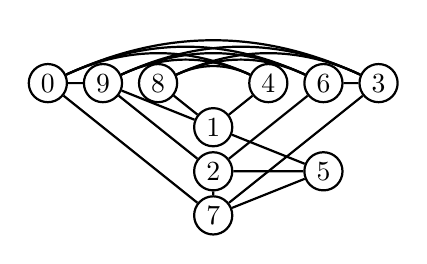
\begin{tikzpicture}[scale=.7,thick, every node/.style={draw, circle, black,inner sep=2pt},yscale=.8]
    \node (0) at (-3,0) {$0$};
    \node (9) at (-2,0) {9};
    \node (8) at (-1,0) {8};
    \node (4) at (1,0) {4};
    \node (6) at (2,0) {6};
    \node (3) at (3,0) {3};
    \node (5) at (2,-2) {5};
    \node (1) at (0,-1) {1};
    \node (2) at (0,-2) {2};
    \node (7) at (0,-3) {7};

    \draw (8) -- (1) -- (9) -- (2) -- (7) -- (0) -- (9);
    \draw (4) -- (1);
    \draw (2) -- (6) -- (3) -- (7);

    \draw[bend left] (0) to (3);
    \draw[bend left] (0) to (4);
    \draw[bend left] (0) to (6);
    \draw[bend left] (9) to (3);
    \draw[bend left] (9) to (4);
    \draw[bend left] (9) to (6);
    \draw[bend left] (8) to (3);
    \draw[bend left] (8) to (4);
    \draw[bend left] (8) to (6);

    \draw (5) -- (1);
    \draw (5) -- (2);
    \draw (5) -- (7);

  \end{tikzpicture}
  \caption{Graph $G_1$, maximum distance obtained between $167$ and $789$.}
  \label{fig}
\end{subfigure}
\begin{subfigure}[b]{0.45\linewidth}
  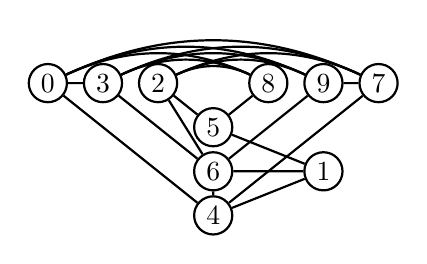
\begin{tikzpicture}[thick, scale=.7,every node/.style={draw, circle, black,inner sep=2pt},yscale=.8]
    \node (0) at (-3,0) {$0$};
    \node (9) at (-2,0) {3};
    \node (8) at (-1,0) {2};
    \node (4) at (1,0) {8};
    \node (6) at (2,0) {9};
    \node (3) at (3,0) {7};
    \node (5) at (2,-2) {1};
    \node (1) at (0,-1) {5};
    \node (2) at (0,-2) {6};
    \node (7) at (0,-3) {4};

    \draw (2) -- (8) -- (1);
    \draw (9) -- (2) -- (7) -- (0) -- (9);
    \draw (4) -- (1);
    \draw (2) -- (6) -- (3) -- (7);

    \draw[bend left] (0) to (3);
    \draw[bend left] (0) to (4);
    \draw[bend left] (0) to (6);
    \draw[bend left] (9) to (3);
    \draw[bend left] (9) to (4);
    \draw[bend left] (9) to (6);
    \draw[bend left] (8) to (3);
    \draw[bend left] (8) to (4);
    \draw[bend left] (8) to (6);

    \draw (5) -- (1);
    \draw (5) -- (2);
    \draw (5) -- (7);

  \end{tikzpicture}
  \caption{Graph $G_2$, maximum distance obtained between $012$ and $056$.}
\end{subfigure}

\begin{subfigure}[b]{0.5\linewidth}
  \centering
  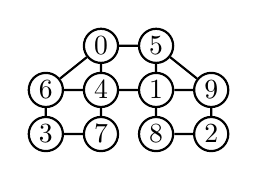
\begin{tikzpicture}[thick, scale=.7,every node/.style={draw, circle, black,inner sep=1.5pt},yscale=.8]
    \node (4) at (0,0) {4};
    \node (1) at (1,0) {1};
    \node (9) at (2,0) {9};
    \node (6) at (-1,0) {6};
    \node (0) at (0,1) {0};
    \node (5) at (1,1) {5};
    \node (3) at (-1,-1) {3};
    \node (7) at (0,-1) {7};
    \node (8) at (1,-1) {8};
    \node (2) at (2,-1) {2};

    \draw (6) -- (3) -- (7) -- (4) -- (6) -- (0) -- (4) -- (1) -- (8) -- (2) -- (9) -- (1) -- (5) -- (9);
    \draw (0) -- (5);
  \end{tikzpicture}

    \caption{Graph $G_3$, maximum distance obtained between $0123$ and $2345$.}
  \end{subfigure}
\end{figure}



\section{Construction for $n=50$ and $n=100$}
The construction for higher number of vertices is based on the graph $G_1$ depicted before. We draw below the reconfiguration graph of $3$-IS in $G_1$.

\begin{figure}[!ht]
  \centering
  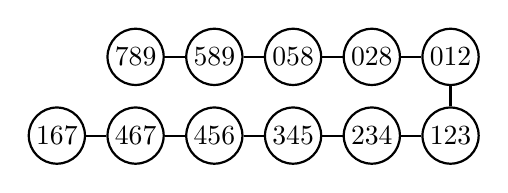
\begin{tikzpicture}[thick,every node/.style={draw, circle, black,inner sep=1.5pt}]
    \node (0) at (0,0) {$789$};
    \node (1) at (1,0) {$589$};
    \node (2) at (2,0) {$058$};
    \node (3) at (3,0) {$028$};
    \node (4) at (4,0) {$012$};
    \node (5) at (0,-1) {$467$};
    \node (6) at (1,-1) {$456$};
    \node (7) at (2,-1) {$345$};
    \node (8) at (3,-1) {$234$};
    \node (9) at (4,-1) {$123$};
    \node (10) at (-1,-1) {$167$};
    \draw (0) -- (1) -- (2) -- (3) -- (4) -- (9) -- (8) -- (7) -- (6) -- (5) -- (10);
    
  \end{tikzpicture}   
  \caption{The reconfiguration graph of $3$-IS in $G_1$.}
  \label{fig2}
\end{figure}

Our construction relies on the following operation. Starting from an instance $(G,\alpha,\beta)$, we construct an instance $(G',\alpha',\beta')$ as follows:
\begin{itemize}
\item Add $10$ new vertices to $G$ inducing $G_1$. We assume that these vertices are labeled with $0,\ldots,9$ according to Figure~\ref{fig}. 
\item For every vertex $u$ of $G$ not in $\alpha$, we add an edge in $G'$ between $u$ and the vertex $1$ of $G_1$. We also add, for every vertex $v \in G$ not in $\beta$ an edge in $G'$ between $v$ and $5$.
\item We set $\alpha'=\alpha\cup \{7,8,9\}$ and $\beta'=\alpha\cup\{7,8,9\}$.
\end{itemize}

We claim that this construction satisfies the following.

  \begin{itemize}
  \item $|V(G')|=|V(G)|+10$;
  \item $|\alpha'|=|\alpha|+3$ and $\alpha'$ is a maximum independent set in $G'$;
  \item The connected component of the reconfiguration graph of $G$ containing $\alpha'$ and $\beta'$ is a path whose endpoints are $\alpha'$ and $\beta'$.
  \item $d'=4d+10$ where $d$ (resp. $d'$) is the distance between $\alpha$ and $\beta$ (resp. $\alpha'$ and $\beta'$) in the reconfiguration graph of $G$ (resp. $G'$).
  \end{itemize}

  The first point is straightforward. The second point also holds. Indeed, $\alpha'$ is a maximum independent set since $\alpha$ is a maximum independent set of $G$ and $G_1$ has independence number $3$. Since $\alpha$ is a maximum independent set of $G$, there must always be three tokens in $G_1$, and these tokens can only move following the reconfiguration sequence of $G_1$. Therefore, at each step, one can either move a token in $G$ (following the reconfiguration graph of $G$) or in $G_1$.
  
  Now observe that tokens in $G_1$ cannot move unless the tokens in $G$ induce $\alpha$ or $\beta$. Conversely, tokens in $G$ cannot move unless the tokens in $G_1$ induce an IS not containing $1$ nor $5$. This ensures that the reconfiguration graph of $G'$ is a path with endpoints $\alpha'$ and $\beta'$. 
  
  One can finally check that the length $d'$ of this path is $4d+10$. In order to put tokens in position $028$ in $G_1$, one needs to put a token in vertex $5$ (see Figure~\ref{fig2}), which implies to put all tokens of $G$ in $\beta$. This requires $d$ steps, hence in $d+3$ steps, we manage to obtain the independent set $\beta\cup\{0,2,8\}$. Now, similarly, to put the tokens on $234$, we need to put tokens in $1$, which requires to put back the tokens of $G$ on $\alpha$. By iterating again this argument twice, we finally obtain a transformation where the total number of token slides in $G$ is $4d$ times, while the total number of token moves in $G_1$ is $10$, which completes the proof. 
  \medskip
  
In particular, applying several times this construction starting from
the instance $(G_1,\{7,8,9\},\{1,6,7\})$, we can construct instances
$(G,\alpha,\beta)$ where $G$ has $n$ vertices, $\alpha,\beta$ are independent sets of size $3n/10$ at distance $\frac{10}{3}(4^{n/10}-1)$ in the
reconfiguration graph (note that their component is a path).

Note that the same construction works when replacing $G_1$ by the complement of a path on $5$ vertices, linking the middle vertex to $\beta$. However, in that case we get $|V(G')|=|V(G)|+5$ and $d'=2d+3$, hence we get graphs on $n$ vertices with a reconfiguration sequence of size $3\times(2^{n/5}-1)$, which is slightly worse. This also means that this construction can be improved with a better choice of $G_1$.
\end{document}
